\section{On-Device Deployment}
\label{sec:deploy}


\subsection{Constraints and design goals}

Our target is the microcontroller inside a battery management system,
which operates without a cloud link, on-device retraining, or an
application processor. That platform imposes two constraints: firmware
alongside protection and balancing logic must not allocate dynamically,
and prediction cost must not grow with the history the operator uses,
because a battery is monitored for its entire service life and that
history only accumulates. Our implementation satisfies the first
directly: freestanding C99, a static pool allocator that reports
exhaustion rather than overrunning its array, and weights held as
const arrays in flash. The focus of this work is not that the model is smaller or faster 
than the baselines at the evaluated window, but rather that its state size does not scale with the window length: 
fixed at $d_k\times d_v$ per layer, it adds only activation scratch, linear in the number of tokens,
whereas a quadratic attention buffer grows with the square of the
context, forcing a larger buffer or a coarser representation of the same
history.

\subsection{Numerical fidelity across architectures}

We implement the full multi-scale model rather than only the single-branch encoder. 
Since both variants share the same GDN-2 kernel implementation, 
the verification established for the encoder extends to the model reported in Section~\ref{sec:exp},
obviating the need for a separate validation argument. 
We compile the same C source for the host and Cortex-M3 and compare the two outputs bit for bit on identical inputs.


\begin{itemize}
\item host C against the PyTorch forward: relative error
  $1.07\times10^{-6}$ for the multi-scale model
  ($2.5\times10^{-6}$ for the single-branch encoder);
\item the Cortex-M3 binary (QEMU mps2-an385, Arm GNU Toolchain
  13.2.rel1) against the host binary: $5.96\times10^{-8}$, about half a
  float32 ULP, for the multi-scale model ($1.19\times10^{-7}$ for the
  encoder).
\end{itemize}

\subsection{Quantization}

Table~\ref{tab:deploy} reports the memory footprints. INT8 yields a $73.4\%$ reduction to 504 KB with no accuracy loss 
(R2=0.9955, MAE=0.00581). INT4 halves this to 268 KB but MAE rises $16.4\%$ (R2=0.9946). 
AE changes from 2.16 to 2.17 cycles, within the ±1.5-cycle seed-to-seed spread. The variants are two deployment tiers: 
multi-scale branches handle three temporal scales; the encoder alone is measured. 
Flash and accuracy drive the choice.

\begin{table}[htbp]
\centering
\caption{Deployed footprints. Weights are the binary payload of the exported
weight arrays; the generated header files are about $3.3\times$ larger,
since the values are written as ASCII text. State is the recurrent matrix
state, fixed and
independent of the window. INT8 and INT4 round per output channel with
fp32 scales. Accuracy is the CALCE SP500 multi-scale model over ten
seeds; the single-branch row is one checkpoint at the same starting
point, and the ten-seed comparison of the two architectures is given in
Table~\ref{tab:ablation}.}
\label{tab:deploy}
\scriptsize
\setlength{\tabcolsep}{3pt}
\begin{tabular}{llrrr}
\toprule
 & & fp32 & INT8 & INT4 \\
\midrule
\multirow{5}{*}{Multi-scale}
 & weights & 1.85\,MB & 504\,KB & 268\,KB \\
 & state (SRAM) & \multicolumn{3}{c}{48\,KB, independent of window} \\
 & $R^2$ & 0.9955 & 0.9955 & 0.9946 \\
 & MAE & 0.00581 & 0.00581 & 0.00676 \\
 & AE (cycles) & 2.16 & 2.17 & 2.40 \\
\midrule
\multirow{4}{*}{Single-branch}
 & weights & 444\,KB & 122\,KB & 67\,KB \\
 & state (SRAM) & \multicolumn{3}{c}{16\,KB} \\
 & AE (cycles) & 1.0 & 0.9 & --- \\
 & & & & \\
\bottomrule
\end{tabular}
\end{table}


\begin{figure}[!ht]
\centering
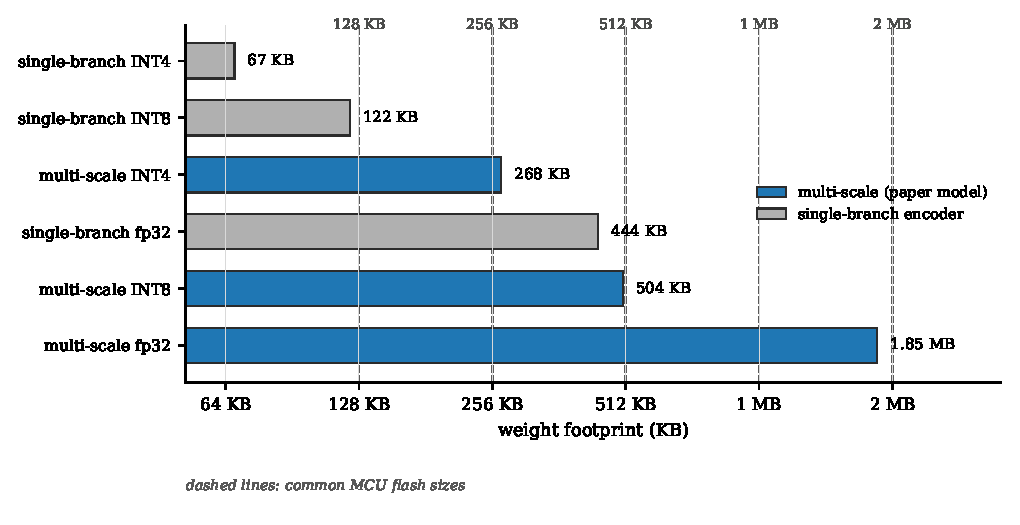
\includegraphics[width=\textwidth]{figures/fig_dep_flash}
\caption{Which precision fits which flash class. Weight footprint at each
(architecture, precision) pair of Table~\ref{tab:deploy}, against the
flash sizes common on Cortex-M parts. The single-branch encoder fits a
$128$\,KB part at INT8 ($122$\,KB) and at INT4 ($67$\,KB); the multi-scale
model needs $512$\,KB at INT4 or INT8 and $2$\,MB at fp32. In every case
the footprint is fixed by the exported weight payload, so the choice can be
made before the part is chosen.}
\label{fig:dep_flash}
\end{figure}

\subsection{Memory and stack budget}

The deployed model's static stack budget is 3.1\,KB, measured with the
compiler's stack-usage report over the whole call chain; nothing is
recursive, nothing is sized at runtime, and the transient activation
buffers come from a pool fixed at compile time. Combined with the fixed
state of Table~\ref{tab:deploy} this means the SRAM requirement is known
at compile time --- the property a safety-related firmware review actually
needs --- and it is why the memory argument can be made without appealing
to any timing measurement.

\subsection{On latency and energy}
\label{sec:latency}

One inference of the full multi-scale model costs
$4.88\times10^{7}$~\mbox{SysTick} ticks on the emulated Cortex-M3, with three
input windows spanning only $0.007\%$ ($48{,}755{,}486$, $48{,}756{,}706$ and
$48{,}753{,}240$). Rebuilt for a core that has a floating-point unit the same
inference costs $3.39\times10^{6}$ ticks, $14.4\times$ fewer. The emulator
measures instructions---$1.95\times10^{9}$, or $1.36\times10^{8}$ with the
FPU---and converting to cycles needs a cycles-per-instruction figure it cannot
supply; at $\mathrm{CPI}\approx1.3$, representative of compiled Thumb-2 on this
core, one inference is $2.54\times10^{9}$ cycles soft-float and
$1.76\times10^{8}$ with the FPU. On the emulator's $25\,\mathrm{MHz}$ those are
$101\,\mathrm{s}$ and $7.1\,\mathrm{s}$; at the $200\,\mathrm{MHz}$ a Cortex-M7
part runs at, the FPU build is $0.9\,\mathrm{s}$. Both are conservative:
$25\,\mathrm{MHz}$ is the MPS2 board's own clock, the Cortex-M3 has no
floating-point unit so every fp32 multiply and add becomes a call into a
software routine, and the FPU figure is a same-core measurement. Because
uniform instruction timing cannot price an FPU instruction's extra cycles,
read $0.9\,\mathrm{s}$ as an estimate and $7.1\,\mathrm{s}$ as the figure the
emulator itself supports.

Energy follows from the same count and is clock-invariant: with core current
$c$ in $\mu\mathrm{A}/\mathrm{MHz}$ and supply $V$, an inference of $N$ cycles
costs
\begin{equation}
E \;=\; c \, V \, N \times 10^{-12}~\mathrm{J}.
\end{equation}
At $c = 300\,\mu\mathrm{A}/\mathrm{MHz}$ and $V = 3.3\,\mathrm{V}$ an
inference costs $2.5\,\mathrm{J}$ soft-float and
$0.17\,\mathrm{J}$ with the FPU; spread over a charge--discharge cycle hours
apart, that is an average draw below a milliwatt. Neither figure changes the
deployment argument, which rests on the memory bound rather than on timing.

\subsection{Comparison with an attention model at equal context}

Figure~\ref{fig:dep_memctx} makes the trade explicit for a model with
$H{=}4$ heads and $d_{\text{model}}{=}64$ attending over $L$ tokens,
against our fixed 48\,KB state.

At the token count our experiments actually use, the attention score
matrix is $16$\,KB --- \emph{smaller} than our state; the crossover is
near $L\approx55$ tokens. By $L{=}1024$ the score matrix alone is
$16$\,MB, $341\times$ our state. The argument is therefore not that a
linear-attention model is cheaper today, but that its cost does not move
when the application needs more context --- and that the KV cache, unlike
the state, keeps growing as inference proceeds.

\begin{figure}[!ht]
\centering

\includegraphics[width=\textwidth]{figures/fig_dep_memctx}
\caption{Working memory against context length, for the same model: the
score matrix ($HL^2\times4$ bytes) and the KV cache
($2Ld_{\text{model}}\times4$ bytes) with $H{=}4$ and
$d_{\text{model}}{=}64$, against the fixed $48$\,KB recurrent state.}
\label{fig:dep_memctx}
\end{figure}

\subsection{Limitations}

Everything above was measured on emulated hardware. The emulator models the
core but not flash wait states or bus contention, so the cycle counts of
Section~\ref{sec:latency} are a lower bound on what a physical part would
spend, and the CPI applied to them is a representative figure rather than a
measured one. No on-device power or thermal measurement is reported.
On-silicon validation is the natural next step and is left to future work.
